\documentclass[12pt]{article}
\usepackage{amsfonts, epsfig}
\usepackage{array}

\usepackage{graphicx}
\usepackage{fancyhdr}
\pagestyle{fancy}
\lhead{Computational Neuroscience - Coursework 2 - Spike Trains}
\rhead{\thepage}
\cfoot{}
\begin{document}

\begin{titlepage}\centering
    \LARGE COMPUTATIONAL NEUROSCIENCE
    \LARGE Coursework 2\\
    \Large Mohamed Nazaal Ibrahim\\
    \Large BSc Mathematics and computer science\\
    \Large Student no. 1636672\\
    \Large University ID. mi16481
\end{titlepage}

\setcounter{secnumdepth}{0}
\section{Question 1}
Suppose that we can simulate spike trains using a Poisson process with a refractory period. We generate a spike train over a 1000 second interval with a firing rate of 35Hz and compute the following statistics for different cases.

\subsection{Fano factor}
The Fano factor $F$ is defined as
\begin{equation}
    F = \frac{\sigma^2}{\mu}
\end{equation}
where $\sigma^2$ is a variance, $\mu$ is an average, both of the spike train. We take these to be the unbiased estimators for the expectation and variance of a given distribution, i.e. make use of the arithmetic mean and arithmetic squared mean. \\
We bin the data into intervals of width 10ms, 50ms and 100ms and compute the Fano factor for the case with no refractory period, and a refractory period of 5ms for each of these intervals.\\
We compute the mean by multiplying the mid-point of the data in each interval with the total count for that interval to get the total and divide this amount by the total count.\\
We compute the variance by first computing the squared mean by squaring the mid-point of the data in each interval before multiplying it with the count for that interval and dividing this by the total count. We then compute the variance as the squared mean minus the mean squared.\\
We then compute the Fano factor for each of the cases as tabulated below.

\begin{center}
    \begin{tabular}{ | m{4cm} | m{2cm}| m{2cm} | m{2cm} | } 
    \hline
    $\#$ & 10ms & 50ms & 100ms \\ 
    \hline
    No refractory  period & 167.55 & 167.54 & 165.39\\ 
    \hline
    Refractory period 5ms & 166.69 & 166.46 & 165.82\\ 
    \hline
    \end{tabular}
\end{center}


\subsection{Coefficient of variation}
The Coefficient of variation is defined as
\begin{equation}
    C_v = \frac{\sigma}{\mu}
\end{equation}
where $\sigma$ is a standard deviation and $\mu$ is an average over the inter-spike interval, i.e. the difference between successive spikes.\\
We first compute the inter-spiker interval sequence, then compute the standard deviation and mean using the functions provided by the numpy library.
\begin{center}
    \begin{tabular}{ | m{4cm} | m{2cm}|  } 
    \hline
    $\#$ &   \\ 
    \hline
    No refractory  period & 1.01 \\ 
    \hline
    Refractory period 5ms & 0.83 \\ 
    \hline
    \end{tabular}
\end{center}

\section{Question 2}
Now we use real data gathered from a fly H1 neuron responding to an approximate white-noise visual motion
stimulus to compute the statistics as in Question 1.
\subsection{Fano factor}
\begin{center}
    \begin{tabular}{ | m{5cm} | m{2cm}| m{2cm} | m{2cm} | } 
    \hline
    $\#$ & 10ms & 50ms & 100ms \\ 
    \hline
    Natural refractory period & 208.69 & 207.05 & 204.51\\ 
    \hline
    \end{tabular}
\end{center}

\subsection{Coefficient of variation}
\begin{center}
    \begin{tabular}{ | m{5cm} | m{2cm}|  } 
    \hline
    $\#$ &   \\ 
    \hline
    Natural refractory period & 2.01 \\ 
    \hline
    \end{tabular}
\end{center}

\section{Question 3}
We now use the motion stimulus that evoked the spike train used in Question 2 to compute the spike triggered average and plot it over a 100ms window.
\begin{center}
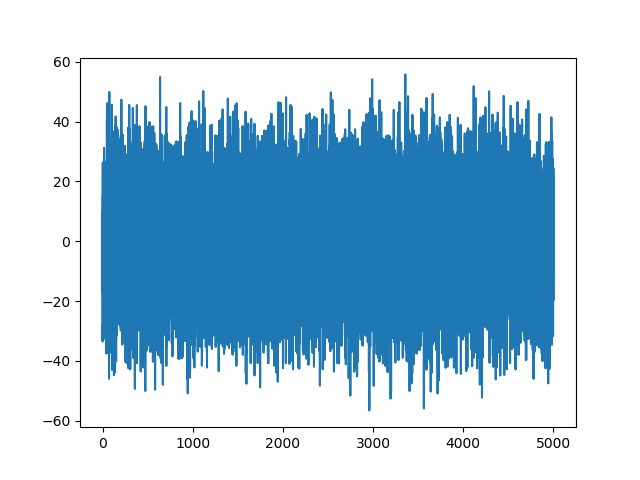
\includegraphics[width=1.\textwidth]{sta.png}
\end{center}


\end{document}
